\documentclass[10pt]{article}
\usepackage[T1]{fontenc}
\usepackage[a4paper,textwidth=122mm,top=18mm,bottom=18mm]{geometry}
\usepackage{graphicx}
\usepackage{tikz}
\usepackage{pgfplots}
\usepackage{pgfplotstable}
\usetikzlibrary{arrows.meta,positioning}
\pgfplotsset{compat=1.18}
\definecolor{rtbdblue}{HTML}{0072B2}
\definecolor{rtbdorange}{HTML}{D55E00}
\definecolor{rtbdgreen}{HTML}{009E73}
\pgfplotsset{rtbdaxis/.style={width=0.95\linewidth,height=0.63\linewidth,
  tick label style={font=\small},label style={font=\small},
  legend style={font=\scriptsize,draw=none,fill=white},
  axis line style={thin},tick align=outside,grid=major,
  grid style={black!12},scaled ticks=false}}
\providecommand{\rtbddatadir}{outputs/figure_data}

\setlength{\parindent}{0pt}
\begin{document}
\begin{center}\large RTBD reproducibility figures\end{center}
\textbf{Filtered completed-case reference.} The following figures reproduce
the completed-case input corpus. The raw-data comparison follows.
\begin{figure}[ht]\centering\begin{tikzpicture}
\begin{axis}[rtbdaxis,xlabel={AGV fleet size},ylabel={Completed products},
  xtick={4,5,6},xmin=3.9,xmax=6.1,ymin=1100,ymax=1460,legend pos=south east]
\addplot[rtbdblue,thick,mark=*] table[x=fleet,y=random,col sep=comma]{\rtbddatadir/throughput_interaction.csv};
\addlegendentry{Random}
\addplot[rtbdorange,thick,dashed,mark=square*] table[x=fleet,y=lwt,col sep=comma]{\rtbddatadir/throughput_interaction.csv};
\addlegendentry{Longest-Waiting-Time}
\addplot[rtbdgreen,thick,dashdotted,mark=triangle*] table[x=fleet,y=nearest,col sep=comma]{\rtbddatadir/throughput_interaction.csv};
\addlegendentry{Nearest-Vehicle}
\end{axis}
\end{tikzpicture}

\caption{Throughput by fleet size and dispatch policy, averaged over the three driving directions.}\end{figure}
\begin{figure}[ht]\centering\begin{tikzpicture}
\begin{axis}[rtbdaxis,xlabel={Maximum production utilization},
  ylabel={Transport-pressure persistence},xmin=0.65,xmax=1.01,ymin=-0.035,ymax=1.04,
  xtick={0.7,0.8,0.9,1.0},ytick={0,0.25,0.5,0.75,1},
  legend style={at={(0.5,-0.27)},anchor=north,legend columns=3,font=\scriptsize,draw=none}]
\addplot[black!40,densely dotted,forget plot] coordinates {(0.9,-0.035) (0.9,1.04)};
\addplot[black!40,densely dotted,forget plot] coordinates {(0.65,0.5) (1.01,0.5)};
\addplot[only marks,rtbdorange,mark=*,mark size=2.5pt,forget plot] table[x=production_utilization,y=transport_persistence,col sep=comma]{\rtbddatadir/landscape_transport_4.csv};
\addplot[only marks,rtbdgreen,mark=*,mark size=2.5pt,forget plot] table[x=production_utilization,y=transport_persistence,col sep=comma]{\rtbddatadir/landscape_mixed_4.csv};
\addplot[only marks,rtbdgreen,mark=square*,mark size=2.5pt,forget plot] table[x=production_utilization,y=transport_persistence,col sep=comma]{\rtbddatadir/landscape_mixed_5.csv};
\addplot[only marks,rtbdblue,mark=*,mark size=2.5pt,forget plot] table[x=production_utilization,y=transport_persistence,col sep=comma]{\rtbddatadir/landscape_production_4.csv};
\addplot[only marks,rtbdblue,mark=square*,mark size=2.5pt,forget plot] table[x=production_utilization,y=transport_persistence,col sep=comma]{\rtbddatadir/landscape_production_5.csv};
\addplot[only marks,rtbdblue,mark=triangle*,mark size=2.5pt,forget plot] table[x=production_utilization,y=transport_persistence,col sep=comma]{\rtbddatadir/landscape_production_6.csv};
\addlegendimage{only marks,mark=*,black}\addlegendentry{4 AGVs}
\addlegendimage{only marks,mark=square*,black}\addlegendentry{5 AGVs}
\addlegendimage{only marks,mark=triangle*,black}\addlegendentry{6 AGVs}
\addlegendimage{only marks,mark=*,rtbdorange}\addlegendentry{Transport pressure}
\addlegendimage{only marks,mark=*,rtbdgreen}\addlegendentry{Mixed pressure}
\addlegendimage{only marks,mark=*,rtbdblue}\addlegendentry{Production pressure}
\end{axis}
\end{tikzpicture}

\caption{RTBD evidence for all 27 filtered logs. Coincident markers can overlap. Colors show the computed regime; production pressure also requires Welding--Painting joint persistence. Dotted lines show the 0.90 saturation and 0.50 transport-persistence cutoffs.}\end{figure}
\clearpage
\textbf{Raw-data sensitivity.} All raw cases are included; unfinished
intervals are right-censored at the 24-hour observation boundary.
\renewcommand{\rtbddatadir}{outputs/figure_data/raw}
\begin{figure}[ht]\centering\begin{tikzpicture}
\begin{axis}[rtbdaxis,xlabel={Maximum production utilization},
  ylabel={Transport-pressure persistence},xmin=0.65,xmax=1.01,ymin=-0.035,ymax=1.04,
  xtick={0.7,0.8,0.9,1.0},ytick={0,0.25,0.5,0.75,1},
  legend style={at={(0.5,-0.27)},anchor=north,legend columns=3,font=\scriptsize,draw=none}]
\addplot[black!40,densely dotted,forget plot] coordinates {(0.9,-0.035) (0.9,1.04)};
\addplot[black!40,densely dotted,forget plot] coordinates {(0.65,0.5) (1.01,0.5)};
\addplot[only marks,rtbdorange,mark=*,mark size=2.5pt,forget plot] table[x=production_utilization,y=transport_persistence,col sep=comma]{\rtbddatadir/landscape_transport_4.csv};
\addplot[only marks,rtbdgreen,mark=*,mark size=2.5pt,forget plot] table[x=production_utilization,y=transport_persistence,col sep=comma]{\rtbddatadir/landscape_mixed_4.csv};
\addplot[only marks,rtbdgreen,mark=square*,mark size=2.5pt,forget plot] table[x=production_utilization,y=transport_persistence,col sep=comma]{\rtbddatadir/landscape_mixed_5.csv};
\addplot[only marks,rtbdblue,mark=*,mark size=2.5pt,forget plot] table[x=production_utilization,y=transport_persistence,col sep=comma]{\rtbddatadir/landscape_production_4.csv};
\addplot[only marks,rtbdblue,mark=square*,mark size=2.5pt,forget plot] table[x=production_utilization,y=transport_persistence,col sep=comma]{\rtbddatadir/landscape_production_5.csv};
\addplot[only marks,rtbdblue,mark=triangle*,mark size=2.5pt,forget plot] table[x=production_utilization,y=transport_persistence,col sep=comma]{\rtbddatadir/landscape_production_6.csv};
\addlegendimage{only marks,mark=*,black}\addlegendentry{4 AGVs}
\addlegendimage{only marks,mark=square*,black}\addlegendentry{5 AGVs}
\addlegendimage{only marks,mark=triangle*,black}\addlegendentry{6 AGVs}
\addlegendimage{only marks,mark=*,rtbdorange}\addlegendentry{Transport pressure}
\addlegendimage{only marks,mark=*,rtbdgreen}\addlegendentry{Mixed pressure}
\addlegendimage{only marks,mark=*,rtbdblue}\addlegendentry{Production pressure}
\end{axis}
\end{tikzpicture}

\caption{Raw-log evidence. Four four-AGV configurations change from transport pressure with low completed-case production exposure to mixed pressure. Throughput is unchanged.}\end{figure}
\renewcommand{\rtbddatadir}{outputs/figure_data}
\begin{figure}[ht]\centering\begin{tikzpicture}
\begin{axis}[rtbdaxis,xlabel={AGV fleet size},ylabel={Blocked fleet capacity (\%)},
  xmin=3.9,xmax=6.1,ymin=-0.3,ymax=8,xtick={4,5,6},legend pos=north east]
\addplot[rtbdblue,thick,mark=*,mark options={fill=white},mark size=3pt] table[x=fleet,y=forward,col sep=comma]{\rtbddatadir/blocking_direction.csv};
\addlegendentry{Forward}
\addplot[rtbdgreen,thick,dashed,mark=x,mark size=2pt] table[x=fleet,y=backward,col sep=comma]{\rtbddatadir/blocking_direction.csv};
\addlegendentry{Backward}
\addplot[rtbdorange,thick,dashdotted,mark=triangle*] table[x=fleet,y=bidirectional,col sep=comma]{\rtbddatadir/blocking_direction.csv};
\addlegendentry{Bidirectional}
\end{axis}
\end{tikzpicture}

\caption{Supplementary filtered-log figure: blocked fleet-capacity time by fleet size and direction. Forward and Backward are both zero.}\end{figure}
\clearpage
\textbf{Original native pipeline.}
\begin{figure}[ht]\centering\resizebox{\linewidth}{!}{%
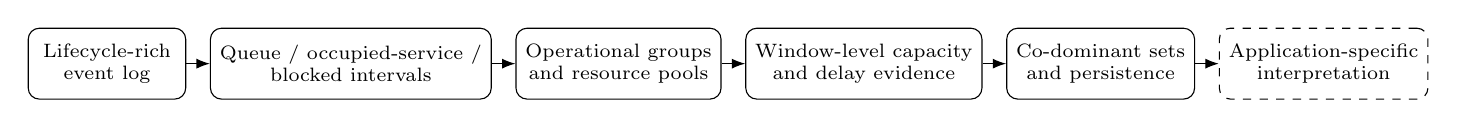
\begin{tikzpicture}[
    node distance=3mm,
    every node/.style={font=\scriptsize,align=center},
    box/.style={
        draw,
        rounded corners,
        minimum width=20mm,
        minimum height=9mm,
        inner sep=1.2mm
    },
    interp/.style={
        draw,
        dashed,
        rounded corners,
        minimum width=20mm,
        minimum height=9mm,
        inner sep=1.2mm
    },
    arr/.style={-{Latex[length=1.7mm]},thin}
]
\node[box] (log) {Lifecycle-rich\\event log};
\node[box,right=of log] (int) {Queue / occupied-service /\\blocked intervals};
\node[box,right=of int] (pool) {Operational groups\\and resource pools};
\node[box,right=of pool] (evid) {Window-level capacity\\and delay evidence};
\node[box,right=of evid] (set) {Co-dominant sets\\and persistence};
\node[interp,right=of set] (regime) {Application-specific\\interpretation};

\draw[arr] (log)--(int);
\draw[arr] (int)--(pool);
\draw[arr] (pool)--(evid);
\draw[arr] (evid)--(set);
\draw[arr] (set)--(regime);
\end{tikzpicture}
}

\caption{Generic measurement layer and application-specific interpretation, retained from the supplied manuscript.}\end{figure}
\end{document}
